\documentclass[12pt]{article}
\nonstopmode
\usepackage{graphicx}
%%\usepackage{times}
%%languaje
\usepackage[spanish]{babel}
\selectlanguage{spanish}
\usepackage[utf8]{inputenc}
\usepackage{hyperref}
\usepackage{fancyhdr}
\usepackage{geometry}
\usepackage{listings}
\usepackage{float}
\usepackage{color}
\usepackage[labelfont=bf]{caption}

\usepackage[square,numbers]{natbib}
\bibliographystyle{unsrtnat}


\usepackage{lipsum}

\usepackage{background}
\backgroundsetup{
    placement=center,
    scale=10,
    contents={DRAFT},
    opacity=1
}
 
 \geometry{
 letterpaper,
 left=3cm,
 right=2cm,
 top=2cm,
 bottom=2cm,
 }

\hypersetup{
	citecolor=black
}

%%colores y formateo XML
\definecolor{maroon}{rgb}{0.5,0,0}
\definecolor{darkgreen}{rgb}{0,0.5,0}
\lstdefinelanguage{XML}
{
  basicstyle=\ttfamily,
  morestring=[s]{"}{"},
  morecomment=[s]{?}{?},
  morecomment=[s]{!--}{--},
  commentstyle=\color{darkgreen},
  moredelim=[s][\color{black}]{>}{<},
  moredelim=[s][\color{red}]{\ }{=},
  stringstyle=\color{blue},
  identifierstyle=\color{maroon}
}



%% quitar guiones cuando las palabras sobrepasan el reglón
\tolerance=1
\emergencystretch=\maxdimen
\hyphenpenalty=10000
\hbadness=10000



\pagestyle{fancy}
\fancyhead{}
\fancyfoot{}
% Set the right side of the footer to be the page number
\fancyfoot[R]{\thepage}


\renewcommand*\rmdefault{iwona}



\hypersetup{colorlinks=true,urlcolor=blue,linkcolor=black}



\begin{document}
\begin{titlepage}


 \vfill
 \begin{minipage}{2.0cm}
     \includegraphics*[width=3.0cm]{img/logo}
 \end{minipage}
 \hfill
 \begin{minipage}{12cm}
 
 \centering
	\textbf{UNIVERSIDAD DE LA FRONTERA}\\
	\textbf{FACULTAD DE INGENIERÍA Y CIENCIAS}\\
	\textbf{DEPTO. CS. COMPUTACIÓN E INFORMÁTICA}
	
 
 \end{minipage}
 
 

	
	\vfill
	
	\textbf{“MINERÍA DE DATOS PARA LOGS DE ALMA COMMON SOFTWARE”}
	\vfill
	
	
	

% Bottom of the page

    \begin{flushright}
	\rule{\linewidth}{.4eX}
	\textbf{
	ANTEPROYECTO DE TRABAJO DE TITULACIÓN\\
	PARA OPTAR AL TÍTULO DE INGENIERO CIVIL INDUSTRIAL MENCIÓN INFORMÁTICA}
	\rule{\linewidth}{.4ex}
	
	\vspace{2cm}
	
	\textbf{Profesor Guía:} DR. PATRICIO ABEL GALEAS ECHEVERRÍA\\
	\textbf{Profesor Co-Guía:} DRA. GLORIA MILLARAY JULIA CURILEM SALDIAS
	
	\end{flushright}
	
	\vspace{1cm}
	\begin{center}
	    \textbf{
	        JAVIER IGNACIO FUENTES MUÑOZ\\
	        2015
	    }
    \end{center}
	
\end{titlepage}

\newpage

\begin{center}
\textbf{ANTEPROYECTO DE TRABAJO DE TITULACIÓN}
\end{center}

\vspace{1cm}

\begin{flushleft}
\textbf{TÍTULO:} MINERÍA DE DATOS PARA LOGS DE ALMA COMMON SOFTWARE\\

\vspace{1cm}

\textbf{NOMBRE:} JAVIER IGNACIO FUENTES MUÑOZ\\

\vspace{1cm}

\textbf{Nº DE MATRÍCULA:} 17627072110\\

\vspace{1cm}

\textbf{CARRERA:} ING. CIVIL INDUSTRIAL MENCIÓN INFORMÁTICA\\

\vspace{1cm}

\textbf{NIVEL CURSADO:} XII

\end{flushleft}

\vfill


\begin{center}
\textbf{JAVIER IGNACIO FUENTES MUÑOZ\\Alumno}
\vspace{1cm}

\textbf{DR. PATRICIO ABEL GALEAS ECHEVERRÍA\\Profesor Guía}
\vspace{1cm}

\textbf{DRA. GLORIA MILLARAY JULIA CURILEM SALDIAS\\Profesor Co-Guía}
\vspace{1cm}

\textbf{MG. NATACHA ALEJANDRA PINO ACUÑA\\Directora de Carrera}

\vspace{1cm}

\textbf{DR. CARLOS FERNANDO CARES GALLARDO\\Director del Departamento}

\end{center}
\vspace{2cm}
\setcounter{page}{0}
\thispagestyle{empty}
\newpage

\tableofcontents

\listoffigures

\lstlistoflistings

\setcounter{page}{0}
\thispagestyle{empty}
\newpage

\section{Acerca de  ALMA}
El proyecto ALMA (Atacama Large Millimeter/submillimeter Array) es un trabajo colaborativo entre el European Southern Observatory (ESO), el National Radio Astronomy Observatory (NRAO) y el National Astronomical Observatory of Japan (NAOJ). Este gran proyecto astronómico consiste en un arreglo de 66 antenas ubicado en el desierto de Atacama, en el norte de Chile.
ALMA tiene como propósito observar el cielo, en búsqueda de nuestros orígenes cósmicos. Esta observación es guiada por científicos y astrónomos del mundo, quienes solicitan espacios de observación.
ALMA Common Software (ACS) provee una plataforma para todos los sistemas del observatorio, la cual se basa en un modelo de componentes de software distribuido. Asimismo, ACS genera un archivo de registros (log) con eventos que dan cuenta del funcionamiento del sistema, tales como: errores, alertas, información de ejecución de programas, interrupciones del sistema, etc.\citep{ESO}.

\subsection{Problemática General}
ACS es un software distribuido altamente complejo. Como toda infraestructura de software, este presenta fallas en su funcionamiento las que pueden llegar a provocar la detención completa del sistema, provocando retrasos en las tareas de observación.
Gran parte del funcionamiento de ACS es permanentemente registrado en archivos de logs, los cuales suman diariamente grandes cantidades de información sobre la operación y eventos asociados a diferentes niveles de alerta. Sin embargo, dada la gran cantidad de registros generados por este sistema, resulta complejo el poder analizar estos datos en forma eficiente y efectiva.
 
Alma tiene un infraestructura altamente compleja, lo que se refleja en sus sistema de generación de logs, por lo que es natural encontrar problemáticas asociadas a numerosas causas y por este motivo es necesario buscar y analizar estas posibles problemáticas. El problema se plantea complejo tanto por la diversidad de los logs como por su cantidad.
 
Por otra parte, se ha desarrollado herramientas y metodologías de minería de datos que tienen por objetivo el apoyar el análisis de grandes volúmenes de datos de manera de poder extraer conocimientos nuevos y útiles. Estas herramientas son capaces de procesar grandes volúmenes de información y encontrar relaciones entre las múltiples variables que afectan los procesos. Para poder aplicar estas herramientas es necesario plantear objetivos de búsqueda y aplicar una metodología de descubrimiento de conocimiento en bases de datos (Knowledge Discovery in Databases, KDD).
 
Sin embargo, debido a la alta complejidad del sistema ACS, los objetivos de búsqueda que guían el análisis son múltiples, lo que requiere de una comprensión muy acabada de todo el proceso para poder modelar algunas partes a través de la minería de datos y buscar entonces las relaciones que permiten comprender por ejemplo, porqué y bajo qué circunstancias el sistema falla. El estudio y comprensión del sistema ACS permitirá la identificación de un problema específico para el cual es posible plantear una aproximación basada en minería de datos.



\newpage

 
\subsection{Objetivo General}

\begin{itemize}
	\item Aplicar metodologías CRISP para generar un modelo de análisis de los LOGS de ACS.
\end{itemize}


\subsection{Objetivos Específicos}
\begin{itemize}	
	\item Identificar un problema relevante para ALMA y que pueda ser abordado analizando los logs del sistema ACS.
	\item Diseñar una metodología basada en CRISP para abordar la problemática identificada.
	\item Crear un prototipo de pre-procesamiento del log de ACS.
\end{itemize}




\section{Antecedentes Generales}

\subsection{ALMA Common Software}
El ALMA Common Software(ACS) es la infraestructura de software, con una arquitectura distribuida e integrada, en donde se manejan todos los procesos del observatorio, desde la captura de los requerimientos para la observación hasta la entrega de los datos capturados \cite{Chiozzi2002}.

Una de las características de ACS es su carácter distribuido, posibilitando que la funcionalidad del sistema pueda implementarse en diferentes lugares geográficos.

Esto hace que ACS sea un sistema heterogéneo, donde diferentes máquinas (hardware) pueden ejecutar software en distintos sistemas operativos y lenguajes de programación. 
El objetivo de un sistema de estas características es que la comunicación entre clientes y servidores sea transparente, independiente de la arquitectura. Esta filosofía de desarrollo se basa en la separación entre la funcionalidad y la arquitectura técnica.
\\
\\
El propósito del \textit{framework} ACS es:
\begin{itemize}
\item Proveer un modelo de programación, para asegurar que una misma función pueda ser desarrollada y ejecutada de la misma forma en cualquier plataforma de desarrollo.
\item Provee interfaces para ser implementadas.
\end{itemize}

ACS provee una filosofía de desarrollo orientado a objetos y los servicios básicos para el cómputo distribuido.

Dentro de estos servicios se encuentran:

\begin{itemize}
\item Invocación remota de objetos transparente.
\item Manejo distribuido de errores y alarmas
\item Manejo distribuido de reporte de eventos (\textit{logging})
\end{itemize}


El \textit{framework} ACS está basado en CORBA\citep{Chiozzi2002}, y está construido en base a código libre.

\subsection{Logs}
\subsubsection{Definición de Log}
Un log es un registro o bitácora que indica la actividad de un sistema. Estos registros o eventos son posteriormente almacenados y tienden a responder el qué, el dónde, el cuándo de un evento particular del sistema \citep{ESOLOG}.


\begin{lstlisting}[label={lst:xml}, caption=Ejemplo un evento XML de log, language=XML]
<Debug TimeStamp="2002-10-7T13:44:16.530"
Host="te1.hq.eso.org" Process="baciTestServer" Thread="main"
Context="" File="baciTestClassImpl.cpp" Line="205"
Routine="BaciTestClass::~BaciTestClass">
    Great debug message!
</Debug>
\end{lstlisting}

Los archivos de Logs son fuentes de valiosa información acerca del estado de un sistema, o de un conjunto de sistemas interconectados. En el listing~\ref{lst:xml} se puede ver un ejemplo de un registro.

Los Logs a procesar son documentos en formato XML. Estos archivos contienen registros que indican información acerca del estado del sistema en forma de eventos. Los eventos, a su vez, contienen datos específicos que describen los detalles asociados al evento en cuestión. Por ejemplo, el instante de tiempo donde ocurre el evento, la máquina que origina, el proceso asociado, entre otros, y además de una descripción en lenguaje natural generada por un programador. 

Todos estos eventos están originalmente clasificados por un tipo que indica el grado de severidad del incidente. Por ejemplo, \textit{Error} , \textit{Warning}, \textit{Info}, \textit{Debug}, \textit{Critical}, etc. \citep{ESOLOG}.


\subsection{Pre-procesamiento de datos}

\subsubsection{Documentos legibles por máquinas}
Uno de los mayores problemas en los archivos de logs es que no están diseñados para el procesamiento automático, sino para ser interpretados por operadores humanos. Por lo tanto, es difícil generar un mecanismo automático para clasificar estos eventos en forma sistemática.


\subsubsection{Tratamientos de texto para los eventos}
Uno de los problemas para poder realizar clasificaciones es que casi todos los eventos son diferentes y es necesario agruparlos según criterios para reducir el número de estos.


Varios de los sistemas de predicción necesitan identificadores numéricos para caracterizar cada tipo de error\citep{Salfner2008a}. En algunos sistemas los eventos incorporan un identificador, y otros simplemente incorporan únicamente información detallada para cada evento, por lo que es necesario realizar algunas de las siguientes operaciones:

\begin{itemize}
\item Separar atributos de cada evento.
\item Remover números en los mensajes.
\item Eliminar atributos vacíos.
\item Transformar el tiempo a formato UNIX
\item \textit{Stemming} de palabras, (reducción a a la raíz de las palabras)
\item Eliminación de conectores en mensajes.
\end{itemize}


Posteriormente de haber tratado los eventos, un algoritmo de clasificación de texto puede generar \textit{clusters}. Algunos de los algoritmos usados para realizar clasificación de documentos de texto son:

\begin{itemize}
\item \textbf{Distancia de Levenshtein}: Este algoritmo calcula la distancia de dos textos, según el mínimo de operaciones requeridas para poder igualar ambos textos. Este valor es útil para poder comparar el parecido de dos mensajes de evento.
\item \textbf{Kmeans - IDF}: Este algoritmo combina dos conceptos diferentes el primero es la matriz inversa de frecuencia de palabras, en otras palabras, la frecuencia de cada termino en un documento, este documento puede ser un mensaje de un evento. El segundo algoritmo kmeans, puede relacionar y agrupar estas frecuencias para determinar clusters con frecuencias similares de los clusters, este algoritmo requiere un tratamiento extra, eliminando conectores y aplicando stemming.
\item \textbf{Locality-sensitive hashing algorithms}: Este tipo de algoritmos permite reducir la dimensionalidad de los datos. Al generar aproximaciones es posible realizar agrupaciones y comparar la similitud entre dos mensajes. Esta clase de algoritmos son utilizados para crear huellas digitales de documentos de video y audio, entre otras aplicaciones.  
\end{itemize}

\subsection{Procesamiento de datos}
Luego de haber pre-procesado los registros, es posible realizar el procesamiento de minería de datos para la búsqueda de patrones. Uno de los algoritmos posibles es:
\subsubsection{SVM}
Las Máquinas de Vectores de Soporte (SVM) abordan problemas de clasificación lineal, mediante la búsqueda de la superficie óptima de separación de dos clases. La superficie óptima, maximiza la distancia entre las dos clases, utilizando los datos más cercanos (vectores de soporte) para construir dicha superficie, como se describe en la Figura \ref{fig:svm} \cite{Cortes1995}. Cuando el problema es no lineal se realiza una proyección de los datos de entrada hacia un espacio llamado ''espacio de características'', generalmente de alta dimensión. Siempre existe un espacio, por más alta que sea su dimensión, en el que es posible encontrar un hiperplano lineal que separa dos clases, como lo muestra la Figura \ref{fig:svm}.

\begin{figure}[H]
\centering
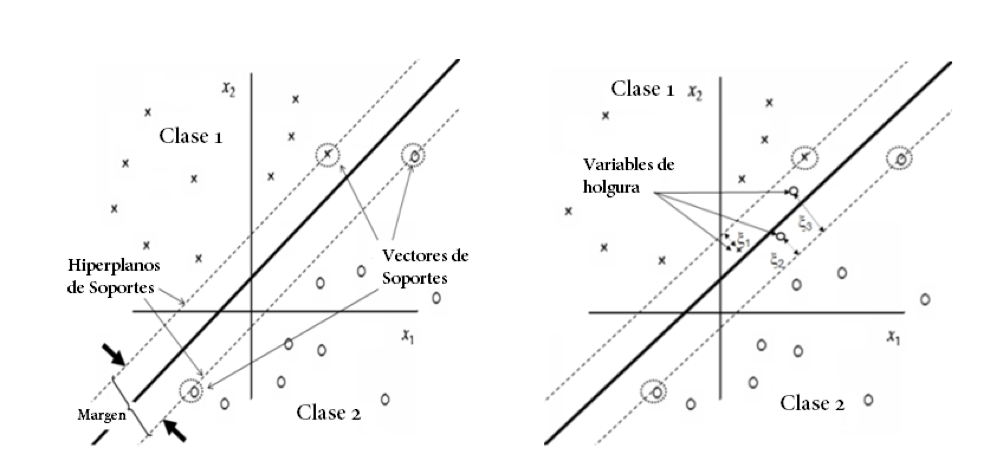
\includegraphics[scale=0.9]{img/svm}
\caption{Hiperplano lineal de separación de dos clases: (\textbf{a}) Margen máximo (\textbf{b}) Margen blando. Los datos destacados con círculos, son vectores de soporte}
\label{fig:svm}
\end{figure}
\newpage
Los parámetros del hiperplano lineal (w, b) se obtienen mediante un algoritmo de optimización que encuentra la mayor distancia (margen) respecto de los vectores de soporte\cite{Scholkopf2001}. Se definen los hiperplanos de apoyo que se muestran en la Figura \ref{fig:svm} (a). Por su parte, la Figura \ref{fig:svm} (b) muestra la situación de margen blando, o sea cuando se permite que algunos puntos crucen los hiperplanos de soporte. Las variables de holgura, son términos que indican en qué medida un punto se encuentra en el lado equivocado de su respectivo hiperplano de soporte. Para resolver problemas no lineales, se utiliza el ''truco del kernel''\cite{Scholkopf2001}. La función de transformación, llamada kernel, proyecta el espacio de entrada en el espacio de características, como se puede observar en la Figura \ref{fig:svm2}.


\begin{figure}[H]
\centering
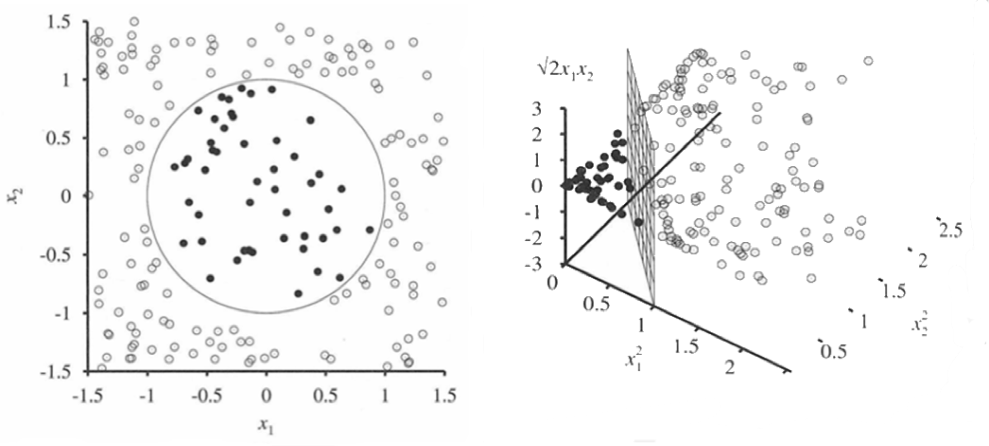
\includegraphics[scale=0.8]{img/svm2}
\caption{Efecto de la asignación del espacio de entrada en un espacio de características dimensional superior, donde es posible un plano de separación lineal.
}
\label{fig:svm2}
\end{figure}


\section{Materiales y Métodos}

\subsection{Metodología}
 
 El propósito de este trabajo es proponer una metodología de minería de datos para logs de ACS. Para esto utilizaremos el proceso de descubrimiento de conocimiento en bases de datos\cite{Fayyad1996}, por sus siglas en inglés \textbf{KDD} (Knowledge Discovery in Databases). Este proceso consta de varias etapas:
 
\begin{enumerate}
	\item Identificación de una problemática a estudiar.
	\item Desarrollo de conocimiento previo del dominio de la aplicación y los objetivos del usuario final.
	\item Creación de un set de datos, en dónde se llevarán a cabo las operaciones.
	\item Limpieza y pre-procesamiento de los datos, eliminación de ruido, estrategias para el manejo de datos faltantes y análisis de las secuencias de tiempo.
	\item Proyección de los datos, búsqueda de características útiles que sean representativas del objetivo del problema. Reducción de los datos, utilizando reducción de dimensionalidad o métodos de transformación para disminuir el número de variables o encontrar una representación invariante para los datos.
	\item Implementación del método de procesamiento de datos.
	\item Búsqueda de patrones utilizando el método escogido, utilizando una representación de interés para reglas de clasificación, regresión, \textit{clustering}.
	\item Interpretación de los datos minados, en caso de que los resultados no sean los esperados es posible volver a iterar cualquiera de los pasos anteriores.
\end{enumerate}


\begin{figure}[H]
\centering
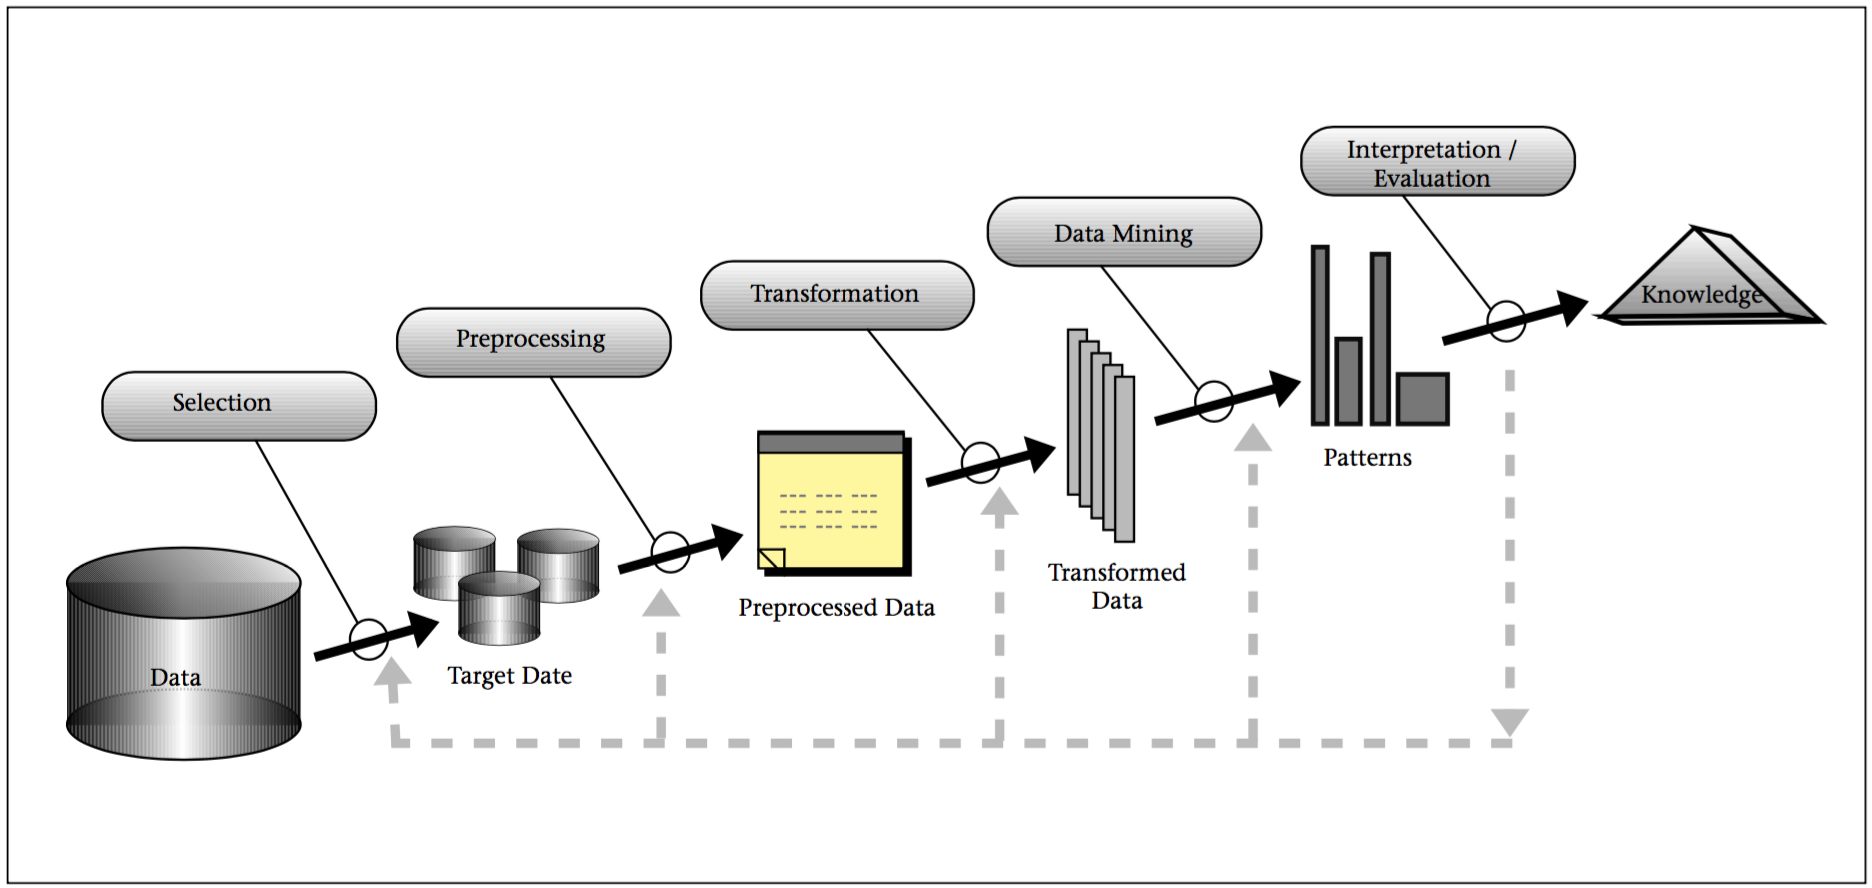
\includegraphics[scale=0.22]{img/kdd}
\caption{Proceso KDD}
\textbf{Fuente}: Fayyad \cite{Fayyad1996}
\end{figure}	



\section{Programa de Trabajo}

\subsection{Descripción de las actividades}

\begin{enumerate}
	\item Identificar en conjunto con el experto de ALMA una problemática contingente al análisis de logs.

	\item Definir los requisitos del problema identificado.

	\item En conjunto con el experto de ALMA, establecer características relevantes en los patrones de LOGs.
	
	\item Implementar una herramienta para la representación visual de las secuencias de log.

	\item Abordar la problemática utilizando la literatura relacionada con el tema de análisis de logs.
	
	\item Identificar una técnica adecuada para enfrentar la problemática.
	
	\item Desarrollar un proceso reducido de \textbf{KDD}, sin iteraciones, basándose en la técnica previamente seleccionada.
	\begin{enumerate}
		\item Selección de un set de datos y operaciones de pre-procesamiento sobre los mismos.
		\item Extracción de características de las secuencias.
		\item Procesamiento de los datos.
		\item Validación de los resultados.
	\end{enumerate}
	
	\item Elaboración del proyecto.
	
\end{enumerate}

\subsection{Carta Gantt}

\begin{figure}[H]
\centering
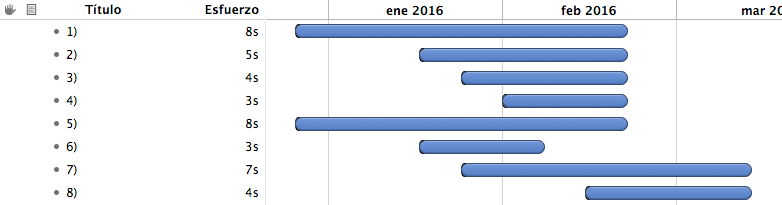
\includegraphics[scale=0.5]{img/gantt}
\caption{Carta Gantt}
\end{figure}


\section{Nomenclatura}
Nomenclaturas utilizadas:
\begin{center}
    \begin{tabular}{ | l |  p{10cm} |}
    \hline
    Evento o registro & Se refiere a cada línea del archivo donde se encuentra el LOG \\ \hline
    LOG &  Documento donde se encuentran todos los eventos \\ \hline
    TAG & Identificador numérico (no único) para cada evento\\ \hline
    Mensaje & Descripción de un evento, escrito en lengueaje naural\\ \hline
    Atributos & Valores que contiene un evento (Tiempo, máquina, etc)\\ \hline
    Tipo de evento & Hace referencia a la categoría de incidencia: Trace (2)
    Delouse
    Debug (3)
    Info (4)
    Notice (5)
    Warning (6)
    Error (8)
    Critical (9)
    Alert (10)
    Emergency (11) \\ \hline
    
    \end{tabular}
\end{center}
\section{Bibliografía}

\bibliography{anteproyecto}


\end{document}